\section{Trading Strategy Design and Performance}
\label{sec:strategy}

\paragraph{Signal.} For each sector, the substitution score is minus the four-quarter change in the QWI junior employment gap; a high score means juniors are losing ground fastest. A quarter's score is used only 12 months after the quarter ends, matching QWI's publication lag. A faster version would use the monthly nowcast (Section~\ref{sec:data}); we report the slow version because it uses only data that were public at the time.

\paragraph{Portfolio.} At the end of each month we rank the 16 sectors on the score and set dollar-neutral rank weights, $w_{s} \propto \operatorname{rank}(\text{score}_s) - \tfrac{N+1}{2}$, scaled to \$1 long and \$1 short, as in \citet{asness2013value}. Rank weights are insensitive to outliers. Weights are held for one month.

\paragraph{Sizing with a weak prior.} We do not know ex ante whether substituting sectors should outperform, so the sign is learned. Each month we update a normal posterior for the strategy's mean return, starting from a prior centered at zero, using only past returns with a five-year half-life (so that a regime change can overturn old evidence). The position is the posterior $z$-score of the mean, clipped to $[-1, 1]$. The strategy can therefore flip from long to short substituting sectors without any look-ahead.

\paragraph{Benchmark and controls.} We compare with a static long-short on AI exposure, the way the market is commonly assumed to trade AI. Each strategy is regressed on the Fama--French five factors \citep{fama2015five}, momentum \citep{carhart1997persistence}, and monthly changes in the 2-year Treasury yield, with Newey--West errors.

\begin{table}[t]
\caption{Backtest, January 1996 to September 2026, monthly. Mean, volatility and alpha are annualized; alpha is the intercept from a regression on the five Fama--French factors, momentum, and the monthly change in the 2-year Treasury yield ($\beta_{2y}$, return per percentage point), with Newey--West $t$-statistics.}
\label{tab:strategy}
\inserttable{tab_strategy}
\end{table}

\begin{figure}[t]
  \centering
  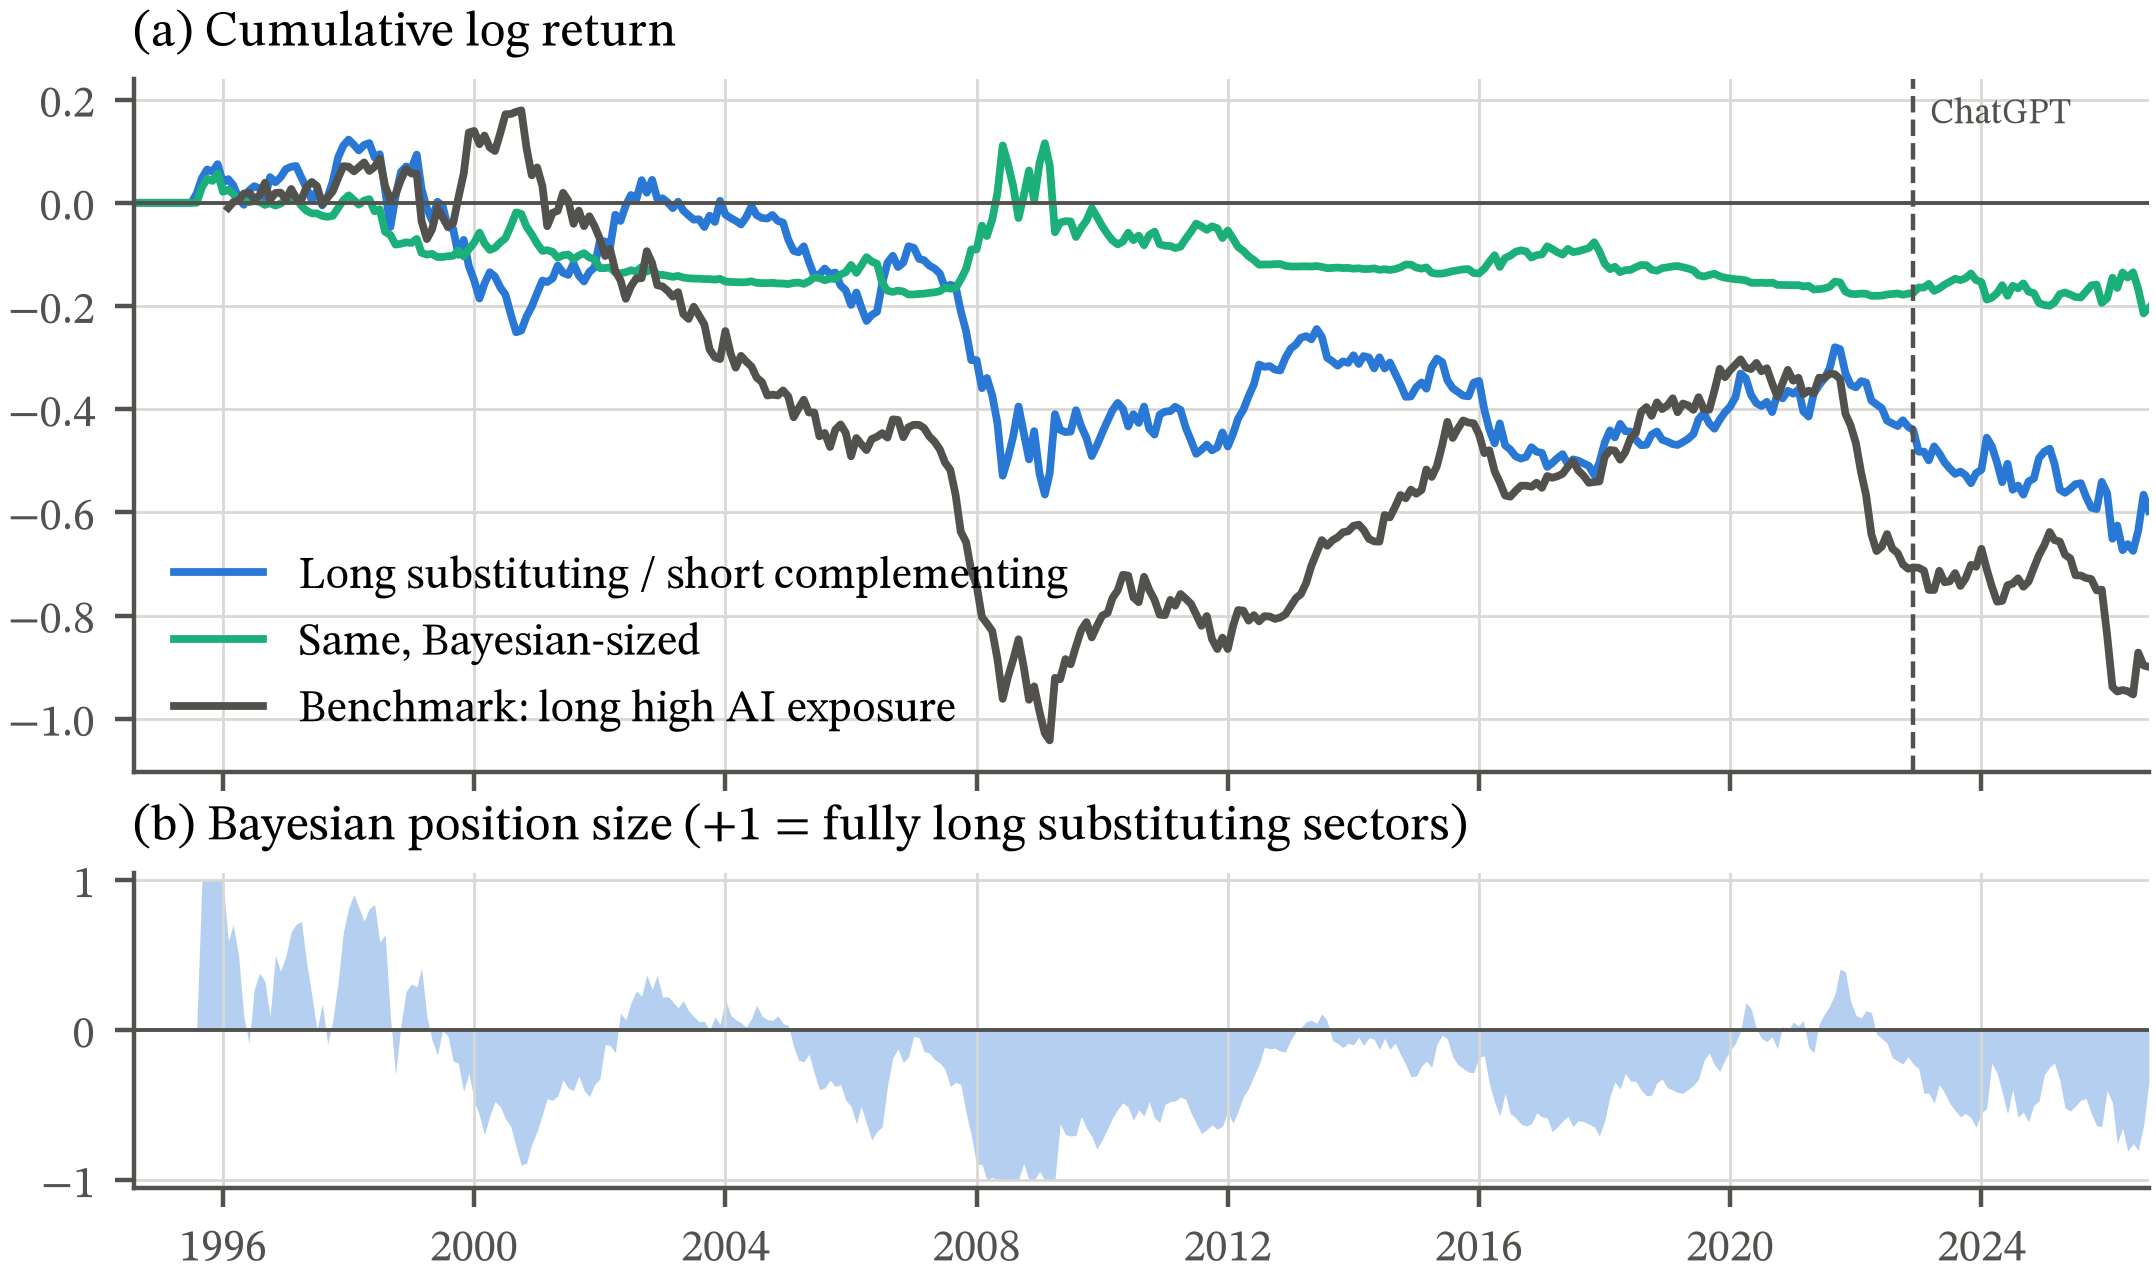
\includegraphics[width=\textwidth]{fig07_strategy.png}
  \caption{(a) Cumulative log returns of the substitution signal, the same signal with Bayesian sizing, and the AI-exposure benchmark. (b) The Bayesian position: $+1$ is fully long substituting sectors, $-1$ fully short.}
  \label{fig:strategy}
\end{figure}

\paragraph{Results.} Table~\ref{tab:strategy} and Figure~\ref{fig:strategy} report the backtest. The substitution signal loses 1.8\% a year with a Sharpe ratio of $-0.19$; its factor-adjusted alpha ($-1.6\%$, $t=-1.0$) is indistinguishable from zero. After ChatGPT the loss widens to 3.6\% a year and the returns load positively on the 2-year yield ($t=2.6$): the long side (substituting sectors) did better when rates rose, which is the discount-rate confound we expected. The Bayesian overlay learns to lean the other way for most of the period after 2000, which cuts volatility to 5.6\% and limits the drawdown to 28\%, but it earns nothing either. The AI-exposure benchmark is worse: $-2.5\%$ a year with a 71\% maximum drawdown, driven by 2008 and by 2022.

\paragraph{Why the result is negative, and why we stand by the analysis.} Three explanations fit the evidence. First, there may be no cash-flow signal to price yet: Section~\ref{sec:results} finds no clear change in the labor share of exposed sectors once the COVID spike is accounted for; and where margins do move, analysts see them quarterly in earnings, well before our 12-month-lagged QWI signal arrives. Second, sector returns are dominated by rate exposure in exactly the sectors we care about; with policy rates moving several hundred basis points in 2022--26, a cash-flow effect of a few percent a year is hard to detect in 16 portfolios. Third, the signal is noisy: turnover is about 127\% a year because quarterly changes in the junior gap are volatile. None of these says the real-side results are wrong. They say the real-side results are not, at sector level and with a one-year lag, a trading edge.

\paragraph{Implementation and risk.} If deployed, we would trade sector ETFs, hedge the 2-year rate exposure with Treasury futures sized by each sector's trailing rate beta, smooth the signal over eight quarters to cut turnover, and use the monthly nowcast to reduce the lag. Position limits and the Bayesian sizing cap drawdowns; the main residual risk is a regime change in rate policy that moves exposed sectors together.
